% ----- formatovani dokumentu -----------------------------------------------
\documentclass[12pt,a4paper,titlepage,final]{report}
\usepackage[utf8]{inputenc}
\usepackage[T1, IL2]{fontenc}
\usepackage{graphicx}
\usepackage{epstopdf}
\usepackage[margin=2cm]{caption}
\usepackage[top=3cm, left=2cm, right=2cm, text={17cm, 24cm}, ignorefoot]{geometry}
\usepackage[usenames,dvipsnames]{color}
\usepackage[]{algorithm2e}
\usepackage{amsmath}

% ------ commands -----------------------


% ---------------------------------------

\usepackage{url}
\usepackage{setspace}
\singlespacing
\usepackage[square, numbers]{natbib} 
\pagestyle{plain}
\pagenumbering{arabic}
\setcounter{page}{1}

\setlength{\parindent}{1cm}	
\usepackage{natbib}
\renewcommand{\thesection}{\arabic{section}}
\renewcommand{\thesubsection}{\arabic{section}.\arabic{subsection}}



% ----- vyberte jazyk -------------------------------------------------------
\usepackage[english,czech]{babel}
%\usepackage[english]{babel}

% ----- dopiste titulky -----------------------------------------------------
\newcommand\Course{Grafické a~multimediální procesory}
\newcommand\WorkTitle{Raytracer na CUDA}
\newcommand\AuthorA{Pavel Macenauer}
\newcommand\AuthorB{Jan Bureš}
\newcommand\AuthorAEmail{xmacen02@stud.fit.vutbr.cz}
\newcommand\AuthorBEmail{xbures19@stud.fit.vutbr.cz}
\newcommand\Faculty{Fakulta Informačních Technologií}
\newcommand\School{Vysoké Učení Technické v~Brně}

\usepackage[
pdftitle={\WorkTitle},
pdfauthor={\AuthorA\AuthorB},
bookmarks=true,
colorlinks=true,
breaklinks=true,
urlcolor=blue,
citecolor=blue,
linkcolor=blue,
unicode=true,
]
{hyperref}



% ----- titulni strana ------------------------------------------------------

\begin{document}
	\begin{titlepage}
	\begin{center}
		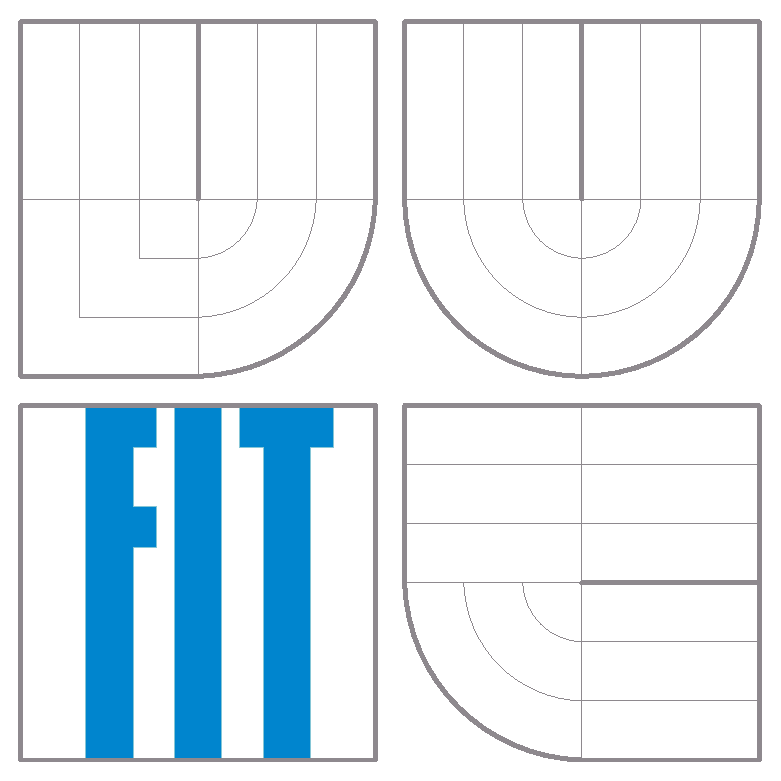
\includegraphics[height=5cm]{images/logo.eps}
	\end{center}
	\vfill
	\begin{center}
		\begin{Large}
			\Course\\
		\end{Large}
		\bigskip
		\begin{Huge}
			\WorkTitle\\
		\end{Huge}
	\end{center}
	\vfill
	\begin{center}
		\begin{large}
			\today
		\end{large}
	\end{center}
	\vfill
	\begin{flushleft}
		\begin{large}
			\begin{tabular}{lll}
				Autor: & \AuthorA, & \url{\AuthorAEmail} \\
				& \AuthorB, & \url{\AuthorBEmail} \\
		
				& & \\
				& \Faculty \\
				& \School \\
			\end{tabular}
		\end{large}
	\end{flushleft}
\end{titlepage}		

\tableofcontents

% ----- obsah -------------------------------------------------------------
\newpage

\section{Zadání}

\begin{itemize}
	\item Implementace Raytraceru pomocí technologie CUDA v~následujícím rozsahu:
	\begin{itemize}
		\item Geometrická primitiva: roviny, koule, trojúhelníky, válce
		\item Načítání modelů z~běžně používaných formátů
		\item Phongův osvětlovací model
		\item Bodové zdroje světla a~stíny
		\item Odlesky
	\end{itemize}
	\item Akcelerace raytracingu na GPU
	\item Vygenerování demonstrační scény a~její vykreslení
	\item Srovnání s~CPU implementací
\end{itemize}

%---------------------------------------------------------------------------
\section{Použité technologie}

Použité technologie:

\begin{itemize}
	\item NVidia CUDA 6.5, \verb!C++!11
	\item Microsoft Visual Studio 2013 + NVidia NSight
	\item GLUT
\end{itemize}

Je přiložen projekt pro Visual Studio (testováno na Microsoft Visual Studio 2013). Pro samotný překlad je pak třeba mít nainstalované NVidia CUDA 6.5. a~používat překladač podporující \verb!C++!11.

%---------------------------------------------------------------------------
\section{Výsledky a~použité znalosti}

\subsection{Srovnání CUDA a~Aurelius raytracerů}

Raytracer jsme testovali ve srovnání s~CPU Raytracerem Aurelius, veřejně dostupným Raytracerem pro předmět PGR.

Oba Raytracery jsou implementovány rozdílně, je tak komplikované vytvořit identické scény. Co ale lze je vytvořit scény podobně komplexní. Vzhled na CUDA raytraceru je mírně kontrastnější a pohled kamery otočen (viz. obrázky \ref{fig:sc-cuda} a \ref{fig:sc-aur}).

\subsection{Testovací scéna}

\begin{figure}
\begin{center}
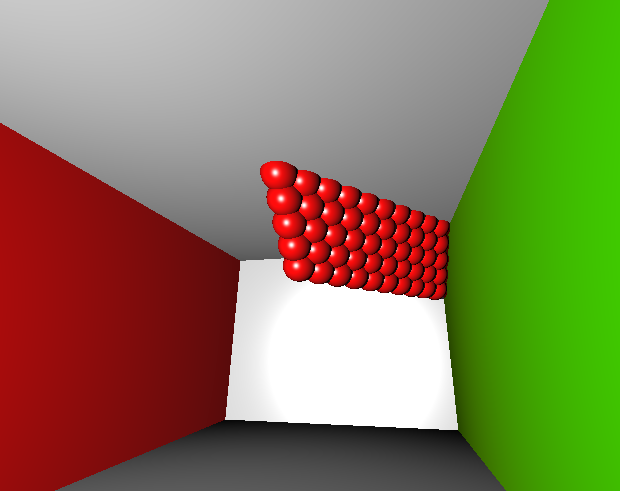
\includegraphics[width=10cm]{images/test-scene.png}
\caption{Testovací scéna na CUDA raytraceru}
\label{fig:sc-cuda}
\end{center}
\end{figure}

\begin{figure}
\begin{center}
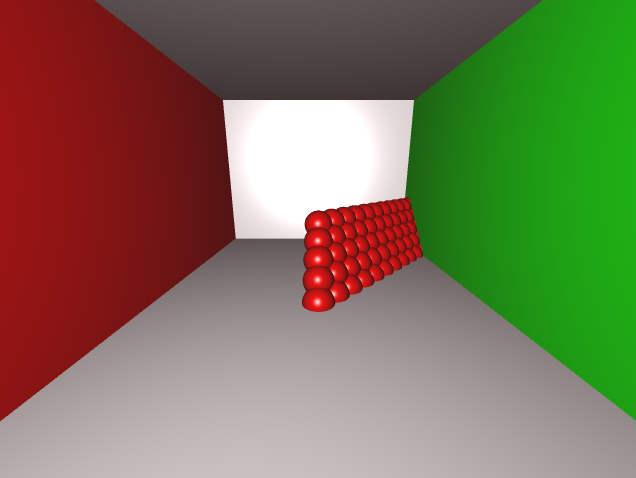
\includegraphics[width=10cm]{images/test-scene-aurelius.png}
\caption{Testovací scéna na raytraceru Aurelius}
\label{fig:sc-aur}
\end{center}
\end{figure}

\begin{itemize}
	\item počet rovin: \textbf{6}
	\item počet koulí: \textbf{5, 10, 20, 50, 100, 500}
	\item hardware: \textbf{NVidia Quadro K1000M, Intel Core i7-3610QM 2.3 GHz}
\end{itemize}

\subsection{Výsledky srovnání}

\begin{figure}
\begin{center}
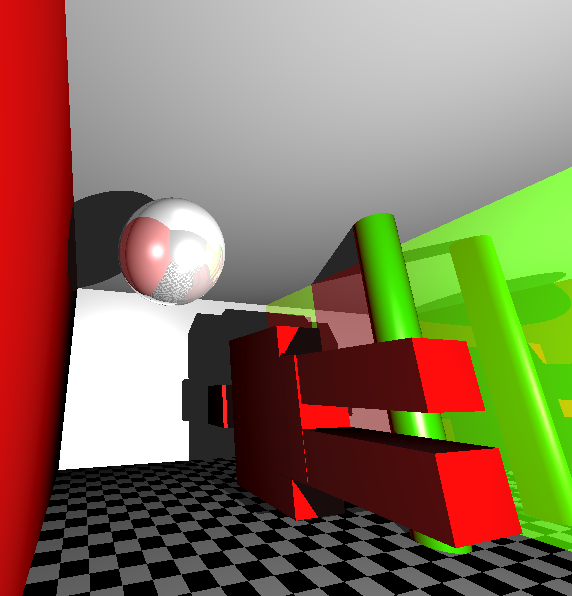
\includegraphics[width=16cm]{images/complex.png}
\caption{Komplexnější scéna obsahující koule, roviny, trojúhelníky a válce s odrazivým materiálem (koule a stěna), procedurálními texturami (šachovnice) a načítáním modelů z obj (ležící panák)}
\end{center}
\end{figure}

\begin{table}
\centering
\begin{tabular}{ | l | l | l | l | l | l | l |}
\hline
\textbf{Počet koulí} & 5  & 10  & 20 & 50 & 100 & 500 \\
\hline
\textbf{CUDA} [s] & 0,0193 & 0,0195 & 0,0224 & 0,0341 & 0,05521 & 0,2197 \\
\hline
\textbf{Aurelius} [s] & 0,905 & 1,233 & 1,779 & 3,541 & 6,505 & 30,373 \\
\hline
\end{tabular}
\caption{Srovnání podobně komplexních scén na raytraceru Aurelius a~CUDA raytraceru pro daný počet koulí}
\end{table}

Syntéza raytracerem Aurelius byla cca 100x pomalejší, než-li syntéza podobné scény na GPU. S~komplexností scény se rozdíly mezi CPU a GPU verzí ještě zvětšují, ale zanedbatelně.


\begin{figure}
\begin{center}
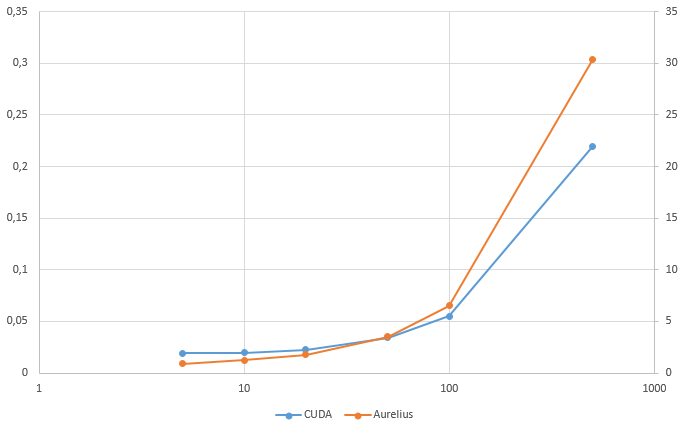
\includegraphics[width=16cm]{images/srovnani.png}
\caption{Srovnání raytraceru Aurelius a~CUDA raytraceru \textit{(osa Y vlevo - doba syntézy pro RT CUDA, osa Y vpravo - doba syntézy pro RT Aurelius)}}
\end{center}
\end{figure}

\subsection{Paralelizace na GPU}

\subsubsection{Rozvržení paměti} 

Raytracer ke svému běhu potřebuje pouze informace o~scéně:
\begin{itemize}
	\item světla (constant memory)
	\item nastavení kamery (constant memory)
	\item informace o~materiálech (constant memory)
	\item databáze primitiv (constant memory)
\end{itemize}

\paragraph{Světla, nastavení kamery a~materiály} jsou data používaná pro výpočet každého paprsku. Zvolili jsme proto uložení v constant memory, která vykazuje nejrychlejší přístupový čas a~zároveň je broadcastována pro všechna vlákna. Diskutabilní může být uložení materiálu pro scény, v případě velkého množství materiálu. Constant memory je nejen omezena velikostí 64 KB, ale je i~z~důvodu broadcastu neefektivní pro scény, kde paprsky budou trefovat primitiva z~různých materiálů.

\paragraph{Databázi primitiv} je vhodné ukládat v~konstantní paměti z~hlediska broadcastu, ale pro scény s~více jak 500-600 primitivy se nevejdeme do max. velikosti constant memory (64 KB), což je i~omezení velikosti scény CUDA raytraceru. Šlo by využít globální paměť, což by však vedlo ke zpomalení.

\subsubsection{Paralelizace výpočtu}

Pro každý pixel syntetizovaného obrazu se vyšle paprsek -- vytvoří vlákno a~to vypočte výslednou barvu (včetně odrazů a~stínů).

\subsection{Optimalizace}

Během implementace jsme tématiku zkoumali a~napadly nás následující optimalizace. Z~časového hlediska, které by často vyžadovaly kompletně přepsat aplikaci a~ve výsledku by nemusely znamenat zlepšení, nejsou z~většiny implementovány.

\subsubsection{Odraz paprsku} 

Při odrazu paprsku od odrazivého materiálu dochází k~vyslání dalšího paprsku. Vlákna, která nic netrefí nebo trefí neodrazivý materiál vracejí výslednou barvu, nicméně stále se musí čekat na vlákna, která se odrážejí. Počítá tak pouze malé množství vláken a~zbytek čeká. 

Nápad na zlepšení je následující:
\begin{enumerate}
	\item Raytracer vyšle paprsek
	\item Zjistí se která vlákna vrátila výsledek (trefila neodrazivý materiál nebo nic) a~která dál chtějí počítat (odrážet se)
	\item Přenese se stav výpočtu zbývajících vláken do paměti
	\item Spustí se kernel pro zbývající vlákna 
\end{enumerate}

\subsubsection{Akcelerační struktury}

CUDA raytracer využívá jako akcelerační struktury KD-tree a~BVH. Nejedná se sice o~rozšíření implementovaná v~rámci rozsahu předmětu GMU, nicméně i~samotné struktury lze optimalizovat.

Intuitivním přístupem je sestavit struktury na CPU a~následně vše nakopírovat na GPU. Struktury je ale možné sestavit i~na GPU, což je mnohem rychlejší. \cite{karras}

\subsection{NVidia CUDA}
Hlavní co jsme museli nastudovat jsou vědomosti ohledně technologie CUDA tedy struktura pamětí, jak je používat pomocí jejího \verb!C++! API a~v~kombinaci s~programováním na CPU.

K~debugování a~programování jsme následně využívali vývojové prostředí Microsoft Visual Studio 2013 s~NVidia NSight.



%---------------------------------------------------------------------------
\section{Ovládání vytvořeného programu}

Raytracer nabízí možnost využití některých akceleračních optimalizací avšak pro tyto optimalizace je nutné raytracer znovu přeložit. Volbu provedeme pomocí podmíněného překladu za použití konstant v~souboru constatns.h. Pro BVH je nutné definovat proměnou ACC\_BVH pomocí "\#define ACC\_BVH". Pro KD-Tree konstantu ACC\_KD\_TREE. Stejně jako optimalizační algoritmy je možné využít různých aplikací raytraceru (neostré  stíny -- OPT\_SOFT\_SHADOWS, hloubka ostrosti -- OPT\_DEPTH\_OF\_FIELD, automaticky pohyb kamery -- OPT\_CAMERA\_SHIFT nebo bilineární samplování -- OPT\_BILINEAR\_SAMPLING). 

V~raytraceru se nastavuje pozice kamery pomocí kláves Q, W, E, A, S, D (A~a~D ve směru osy~x, W a~S~ve směru osy~y, Q a~E ve směru osy~z) avšak bod, na který kamera směřuje se nezmění. Pokud raytracer přeložíte pro výpočet hloubky ostrosti můžete měnit ohniskovou vzdálenost pomocí R a T.

Komplexnější scény zapsané ve formátu OBJ je možné v~ratraceru zobrazit tak, že soubor s~koncovkou obj vložíme do složky, ze které raytracer spouštíme.  


%---------------------------------------------------------------------------
\section{Rozdělení práce v~týmu}

Oba jsme pracovali na všem, nicméně specializovali jsme se následovně:

\begin{itemize}
\item \textbf{Jan Bureš}: Phongův osvětlovací model, úprava bilineární interpolace, hloubka ostrosti, měkké stíny, válec, trojúhelník, rovina, především raytracing-části raytraceru\dots
\item \textbf{Pavel Macenauer}: Základní kostra programu, optimalizace využitých paměťových jednotek, základ pro bilineární interpolaci, načítání formátu OBJ, akcelerační struktury, především CUDA-části raytraceru\dots
\end{itemize}

%---------------------------------------------------------------------------
\section{Co bylo nejpracnější}

\begin{itemize}
\item \textbf{Jan Bureš}: Na celé práci bylo asi nejsložitější upravit algoritmus sledování paprsku tak, aby fungoval na architektuře CUDA. Dále pak správné rozdělení vláken do warpů a~rozhodnout, který druh paměti použít pro které proměnné. Mnoho času bylo zapotřebí také věnovat rekurzi, kterou by sice CUDA měla podporovat od verze 3.0, ovšem stále program havaroval kvůli přetečení zásobníku.

\item \textbf{Pavel Macenauer}:  Celkové zprovoznění CUDA a navázání na OpenGL + následné vykreslení. To především proto, že dokumentace a~materiály jsou především v~podobě vygenerované dokumentace od společnosti NVidia a~materiálů na internetu k~této tématice moc není. Dále i~parsování souboru OBJ a~vkládání jednotlivých trojúhelníku do paměti.
\end{itemize}
%---------------------------------------------------------------------------
\section{Zkušenosti získané řešením projektu}

Naučili jsme se více o~architektuře CUDA, získali představu o~psaní paralelních algoritmů a~optimalizovali značně rychlost výpočtu. Zdokonalili jsme raytracer do podoby, kdy již nevykresluje jen koule, ale i~komplexnější scény, odráží paprsky. Optimalizovali jsme rychlost, vyzkoušeli si implementovat phongův osvětlovací model a~raytracer v~praxi. Prostudovali možné algoritmické optimalizace raytraceru a~některé z~nich implementovali.


%---------------------------------------------------------------------------
\section{Autoevaluace}

\paragraph{Technický návrh (85\%):} 
Tvorbu programu jsme si naplánovali na jednotlivé iterace, a~tak až na pár úprav, které nás napadli během implementace nebylo nutné přepisovat již implementované části. Především se jednalo o~části týkající se správy paměti, kdy s~každým typem paměti na GPU se pracuje trochu jinak.

\paragraph{Programování (75\%):}
Kód je dobře strukturovaný, ale mohl by být více okomentován, např. pro vygenerování použitelné doxygen dokumentace. 
Implementovaný raytracer je možné rozšiřovat a~bez sebevětších komplikací přidávat další doplňky.

\paragraph{Vzhled vytvořeného řešení (80\%):} 
Scéna vypadá celkem pěkně. Jednotlivá primitiva mají ostré hrany, tak by neuškodilo implementovat antialiasing. Některé optimalizace kvalitu obrazu mírně zhorší, ale vždy dle očekávání. 

\paragraph{Využití zdrojů (90\%):}
Hodně jsme využili již implementovaný raytracer Aurelius k~lepšímu pochopení raytracingu a~trochu méně pak dostupnou literaturu. Zdroje o~CUDě a~jejím zapojení jsme získali především z~vyhledávače Google.

\paragraph{Hospodaření s~časem (70\%):}
Na raytraceru jsme pracovali průběžně, využití GIT repositáře umožnilo, že jsme vždy každou volnou chvíli něco málo naimplementovali. Uprostřed semestru naše snaha mírně opadla kvůli jiným povinnostem ve škole. Na závěr jsme se snažili vše dokončit v~čas, což se i~povedlo.

\paragraph{Spolupráce v~týmu (95\%):}
Od začátku jsme komunikovali ohledně podmínek spolupráce. Následné programování pak probíhalo bez problémů a~o~všem jsem se navzájem informovali přes instantní mluvítka jako Skype nebo Facebook. Veškeré změny jsme pak evidovali v~repositáři na serveru GitHub.com, kde jsme i~vybudovali společné vývojové prostředí.

\paragraph{Celkový dojem (90\%):} 

S~raytracingem se setkáváme ve více předmětech, proto jsme projekt kombinovali i~s~předmětem PGP, pro který byly implementovány akcelerační struktury. Celý projekt už je celkem komplexní a~jednoznačně nad rámec jednoho předmětu. Nejedná se již o~jednoduchý GPU raytracer, ale raytracer schopný vykreslovat různé druhy primitiv, modely, využívá různé druhy akcelerace a~rozšiřující vizuální aplikace.

Projekt je celkově zajímavý tím, že se jedná o~komplexní raytracer, který se postupně formuje do podoby raytracingového enginu/frameworku. Na rozdíl od velkého množství projektů, které zmizí v propadlišti dějin, se jedná o~práci, která by i~mohla zaujmout své jedinečné místo na internetu.


%---------------------------------------------------------------------------
\section{Doporučení pro budoucí zadávání projektů}

\begin{itemize}
	\item Zveřejnit zadání pro projekty již od 1. týdne - umožní to nastudovat tématiku dopředu a~vytvořit tak prostor pro diskuzi na přednáškách. Navíc na začátku semestru je nejvíce času, dále pak jsou úkoly, půlsemestrální písemky a~je možné se vyhnout práci na poslední chvíli.
	\item Kostry pro jednotlivé projekty. Některé projekty se zpracovávají během let opakovaně. Určitě by tak pro ně šlo vytvořit kostry (něco jako pro domácí úkoly), které by umožňovali odstranit onu část vše rozchodit, nainstalovat, napsat základy a~věnovat se komplexnějším věcem. Umožnilo by to i~lehčí kontrolu pro vyučující.
\end{itemize}

%---------------------------------------------------------------------------

\bibliographystyle{plain}

\nocite{pgr-raytracing}
\nocite{aurelius}
\nocite{pgp-optimalizace}
\nocite{cuda-doc}
\nocite{phong-wiki}
\nocite{so-stack}
\nocite{bvh}
\nocite{cmemory}
\nocite{trier}
\nocite{STRACHOTA}
\nocite{HART}
\nocite{COOK}
\nocite{STOCHASTIC}
\nocite{FUSSELL}



\bibliography{reference}
\addcontentsline{toc}{section}{Literatura}


\end{document}

